\section{Einleitung}
\label{sec:einleitung}

List Example:
\begin{itemize}
\item Maximaler Schub beim Starten z.B. wegen kurzer Startbahn
\item Maximale Fluggeschwindigkeit erreichen z.B. bei Rettungsflügen oder Ähnlichem
\item Maximale Effizienz z.B. um möglichst lange Flugzeiten zu ermöglichen
\end{itemize}



Bild Beispiel:
\vspace{0.05cm}

\begin{figure}[htb!]
	\begin{center}
		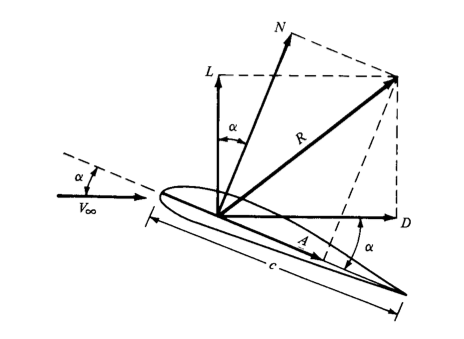
\includegraphics[width=0.48\textwidth]{airfoilKraefte}
		\caption[Wirksame aerodynamische Kräfte an einem Profil]{Wirksame aerodynamische Kräfte an einem Profil \cite{aeroKraefte}. Die Auftriebskraft $L$ wirkt beim Propeller als Schub und die Widerstandskraft $D$ als Drehmoment.}
		\label{fig:airfoilKraefte}
	\end{center}
\end{figure}

\vspace{0.05cm}

Unterkapittel:

\subsection{Subsection test}
\label{subsec:speichernderresultatematlab}

Wenn die Propellerberechnung beendet ist, werden alle Resultate in eine Baumstruktur gespeichert. Somit sind die Resultate schnell wieder aufrufbar und auch sauber in einer einzigen Datei geordnet und gespeichert.\\

\subsubsection{Subsubsection test}
\label{subsubsec:speichernderresultatematla2}

Wenn die Propellerberechnung beendet ist, werden alle Resultate in eine Baumstruktur gespeichert. Somit sind die Resultate schnell wieder aufrufbar und auch sauber in einer einzigen Datei geordnet und gespeichert.\\

\subsubsection{Subsubsubsection test}
\label{subsubsec:speichernderresultatematlab3}

Wenn die Propellerberechnung beendet ist, werden alle Resultate in eine Baumstruktur gespeichert. Somit sind die Resultate schnell wieder aufrufbar und auch sauber in einer einzigen Datei geordnet und gespeichert.\\

\newpage

